\begin{figure}
 \centering
 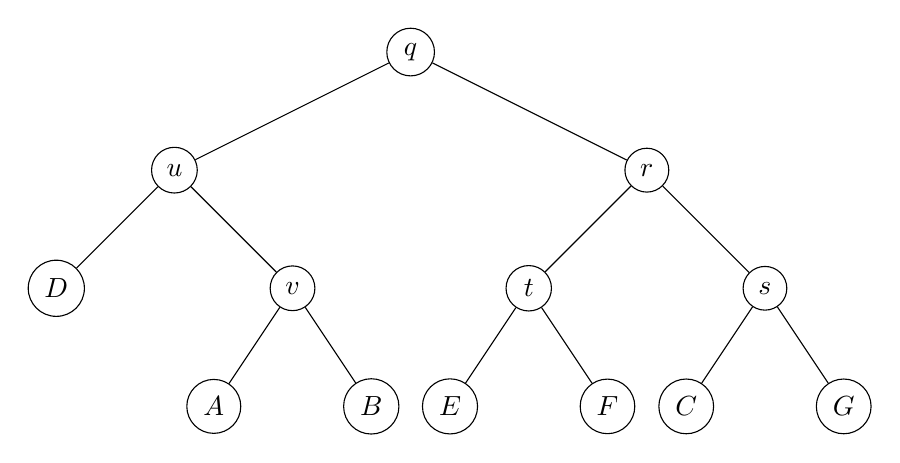
\begin{tikzpicture}[level/.style={sibling distance = 60mm/#1}]
  \node[circle,draw] (z){$q$}
   child {node [circle,draw] (a) {$u$}
    child {node [circle,draw] (b) {$D$}}
    child {node [circle,draw] (c) {$v$}
     child {node [circle,draw] (d) {$A$}}
     child {node [circle,draw] (e) {$B$}}
    }
   }
   child {node [circle,draw] (f) {$r$}
    child {node [circle,draw] (g) {$t$}
     child {node [circle,draw] (h) {$E$}}
     child {node [circle,draw] (i) {$F$}}
    }
    child {node [circle,draw] (j) {$s$}
     child {node [circle,draw] (k) {$C$}}
     child {node [circle,draw] (l) {$G$}}
    }
  };
 \end{tikzpicture}
 \caption{Tasosta muodostettu kd-puu}
 \label{bsp4}
\end{figure}
